\chapter{Machine à vecteurs de support}

\myminitoc

\sect{Machines d'apprentissage linéaire}

On reprend un apprentissage linéaire qui consiste à trouver un hyperplan $\langle w, x \rangle + b = 0$ qui sépare deux classes $-1$ et $1$. Pour cela on dispose de données d'entraînements $T = \left\{ (x_i, y_i) \right\}_{i=1}^n$. Les paramètres $w$ et $b$ peuvent être appris par un perceptron par exemple.

\DEF{
	La \textbf{marge} d'une instance $z_i = (x_i, y_i)$ par rapport à l'hyperplan de direction $w$ et de biais $b$ est définie par :
	$$ \gamma_i = y_i \left( \langle w, x_i \rangle + b \right) $$
	Puis la marge de l'hyperplan respectivement à l'ensemble d'entraînement $T$ est :
	\vspace{-2mm}
	$$ \gamma = \min_{1 \leqslant i \leqslant n} \gamma_i = \min_{(x, y) \in T} y \left( \langle w, x \rangle + b \right) $$
	\vspace{-5mm}
}

\REM{
	La marge est positive si $z_i$ est correctement classé. \\
	La distance de $x_i$ à l'hyperplan est $ \dfrac{| \langle w, x_i \rangle + b |}{\| w \|}$. Ainsi la marge représente une distance euclidienne signée.
}

\begin{center}
	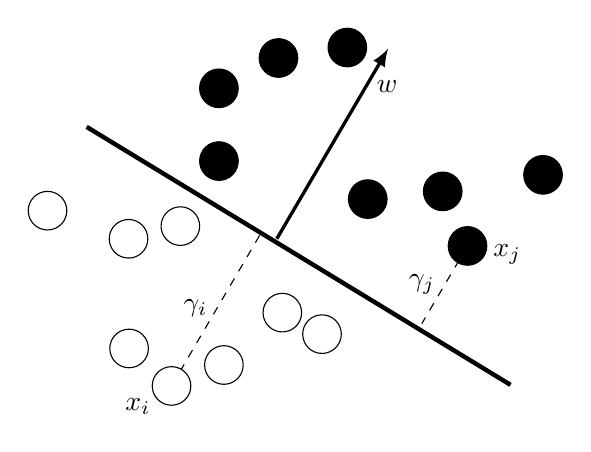
\begin{tikzpicture}[>={latex}, scale=0.7]
		\draw[dashed] (6.98, -2.04) -- node[left] {$\gamma_j$} (6.15, -3.45);
		\node at (7.7, -2.2) {$x_j$};
		\draw[dashed] (1.61, -4.58) -- node[left] {$\gamma_i$} (3.26, -1.76);
		\node at (1, -4.95) {$x_i$};
		\draw[very thick, ->] (3.52, -1.91) -- node[pos=0.8, right] {$w$} (5.54, 1.54);
		\draw[ultra thick] (0.07, 0.12) -- (7.76, -4.56);
		\draw[fill=black] (6.98, -2.04) circle (0.35);
		\draw[fill=black] (6.53, -1.05) circle (0.35);
		\draw[fill=black] (8.35, -0.75) circle (0.35);
		\draw[fill=black] (5.17, -1.19) circle (0.35);
		\draw[fill=black] (2.47, -0.50) circle (0.35);
		\draw[fill=black] (4.80, 1.56) circle (0.35);
		\draw[fill=black] (3.55, 1.37) circle (0.35);
		\draw[fill=black] (2.47, 0.82) circle (0.35);
		\draw[fill=white] (1.77, -1.68) circle (0.35);
		\draw[fill=white] (1.61, -4.58) circle (0.35);
		\draw[fill=white] (0.83, -1.91) circle (0.35);
		\draw[fill=white] (-0.64, -1.40) circle (0.35);
		\draw[fill=white] (3.62, -3.25) circle (0.35);
		\draw[fill=white] (4.34, -3.64) circle (0.35);
		\draw[fill=white] (2.56, -4.20) circle (0.35);
		\draw[fill=white] (0.84, -3.90) circle (0.35);	
	\end{tikzpicture}
\end{center}

\paragraph{Dual}
L'algorithme perceptron construit $w$ en ajoutant itérativement des instance mal classés. Ainsi le vecteur $w$ obtenu est une combinaison linéaire des instances d'entraînement.
$$ w = \sum_{i=1}^n \alpha_i y_i x_i $$
Où les $\alpha_i$ sont positif et proportionnels au nombre de fois où l'exemple $x_i$ a été mal classé. Ainsi les exemples difficiles ont une valeur $\alpha_i$ élevée. Finalement l'apprentissage a juste besoin des produits scalaires entre les différents exemples. La matrice $G$ définie par {\boldmath $G_{ij} = \langle x_i, x_j \rangle$} est la \textbf{matrice de Gram}.

\sect{Astuce du noyau}

L'apprentissage linéaire ne peux pas traiter des cas de séparation non linéaire. On pourrait travailler avec des modèles plus complexes mais ce n'est pas dans la philosophie du rasoir d'Occam. On cherche un modèle simple. On va donc garder une classification linéaire mais on va essayer d'utiliser un espace des features plus adéquat. Voici la stratégie :
\begin{itemize}
	\item Utiliser une transformation non linéaire $\Phi : \X \rightarrow \mathcal{F}$ pour projeter les données dans un nouvel espace $\mathcal{F}$.
	\item Apprendre une séparation linéaire sur $\mathcal{F}$.
\end{itemize}

\begin{center}
	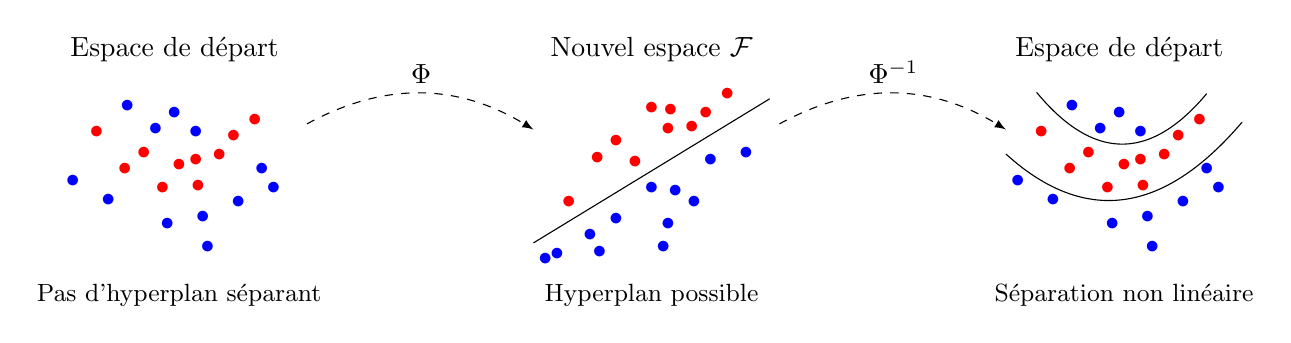
\begin{tikzpicture}[>={latex}, scale=3]
		\node at (0.5, 0.94) {Espace de départ $\X$};
		\node at (0.5, -0.1) {\small Pas d'hyperplan séparant};
		
		\node[blue] at (0.28, 0.7) {$\bullet$};
		\node[blue] at (0.4, 0.6) {$\bullet$};
		\node[blue] at (0.48, 0.67) {$\bullet$};
		\node[blue] at (0.57, 0.59) {$\bullet$};
		\node[blue] at (0.05, 0.38) {$\bullet$};
		\node[blue] at (0.2, 0.3) {$\bullet$};
		\node[blue] at (0.45, 0.2) {$\bullet$};
		\node[blue] at (0.62, 0.1) {$\bullet$};
		\node[blue] at (0.6, 0.23) {$\bullet$};
		\node[blue] at (0.75, 0.29) {$\bullet$};
		\node[blue] at (0.85, 0.43) {$\bullet$};
		\node[blue] at (0.9, 0.35) {$\bullet$};
		
		\node[red] at (0.15, 0.59) {$\bullet$};
		\node[red] at (0.27, 0.43) {$\bullet$};
		\node[red] at (0.35, 0.5) {$\bullet$};
		\node[red] at (0.43, 0.35) {$\bullet$};
		\node[red] at (0.5, 0.45) {$\bullet$};
		\node[red] at (0.57, 0.47) {$\bullet$};
		\node[red] at (0.58, 0.36) {$\bullet$};
		\node[red] at (0.67, 0.49) {$\bullet$};
		\node[red] at (0.73, 0.57) {$\bullet$};
		\node[red] at (0.82, 0.64) {$\bullet$};
		
		\node (x) at (1, 0.6) {};
		\draw[dashed, ->] (x) edge[bend left] node[above] {$\Phi$} (2, 0.6);
		\node at (2.5, 0.94) {Nouvel espace $\mathcal{F}$};
		\node at (2.5, -0.1) {\small Hyperplan possible};
		\draw (2, 0.12) -- (3, 0.73);
		
		\node[blue] at (2.05, 0.05) {$\bullet$};
		\node[blue] at (2.1, 0.07) {$\bullet$};
		\node[blue] at (2.24, 0.15) {$\bullet$};
		\node[blue] at (2.28, 0.08) {$\bullet$};
		\node[blue] at (2.35, 0.22) {$\bullet$};
		\node[blue] at (2.5, 0.35) {$\bullet$};
		\node[blue] at (2.55, 0.1) {$\bullet$};
		\node[blue] at (2.57, 0.2) {$\bullet$};
		\node[blue] at (2.6, 0.34) {$\bullet$};
		\node[blue] at (2.68, 0.29) {$\bullet$};
		\node[blue] at (2.75, 0.47) {$\bullet$};
		\node[blue] at (2.9, 0.5) {$\bullet$};
		
		\node[red] at (2.15, 0.29) {$\bullet$};
		\node[red] at (2.27, 0.48) {$\bullet$};
		\node[red] at (2.35, 0.55) {$\bullet$};
		\node[red] at (2.43, 0.46) {$\bullet$};
		\node[red] at (2.5, 0.69) {$\bullet$};
		\node[red] at (2.57, 0.6) {$\bullet$};
		\node[red] at (2.58, 0.68) {$\bullet$};
		\node[red] at (2.67, 0.61) {$\bullet$};
		\node[red] at (2.73, 0.67) {$\bullet$};
		\node[red] at (2.82, 0.75) {$\bullet$};
		
		\node (x) at (3, 0.6) {};
		\draw[dashed, ->] (x) edge[bend left] node[above] {$\Phi^{-1}$} (4, 0.6);
		\node at (4.5, 0.94) {Espace de départ $\X$};
		\node at (4.5, -0.1) {\small Séparation non linéaire};
		
		\node[blue] at (4.28, 0.7) {$\bullet$};
		\node[blue] at (4.4, 0.6) {$\bullet$};
		\node[blue] at (4.48, 0.67) {$\bullet$};
		\node[blue] at (4.57, 0.59) {$\bullet$};
		\node[blue] at (4.05, 0.38) {$\bullet$};
		\node[blue] at (4.2, 0.3) {$\bullet$};
		\node[blue] at (4.45, 0.2) {$\bullet$};
		\node[blue] at (4.62, 0.1) {$\bullet$};
		\node[blue] at (4.6, 0.23) {$\bullet$};
		\node[blue] at (4.75, 0.29) {$\bullet$};
		\node[blue] at (4.85, 0.43) {$\bullet$};
		\node[blue] at (4.9, 0.35) {$\bullet$};
		
		\node[red] at (4.15, 0.59) {$\bullet$};
		\node[red] at (4.27, 0.43) {$\bullet$};
		\node[red] at (4.35, 0.5) {$\bullet$};
		\node[red] at (4.43, 0.35) {$\bullet$};
		\node[red] at (4.5, 0.45) {$\bullet$};
		\node[red] at (4.57, 0.47) {$\bullet$};
		\node[red] at (4.58, 0.36) {$\bullet$};
		\node[red] at (4.67, 0.49) {$\bullet$};
		\node[red] at (4.73, 0.57) {$\bullet$};
		\node[red] at (4.82, 0.64) {$\bullet$};
		
		\draw[domain=0:1, smooth, variable=\x]
		plot({\x+4}, {(\x - 0.56)^2 * 1.04 + 0.17 + 0.26 * \x});
		\draw[domain=0.13:0.85, smooth, variable=\x]
		plot({\x+4}, {(\x - 0.63)^2 * 1.67 + 0.28 + 0.46 * \x});
	\end{tikzpicture}
\end{center}

Notre classificateur s'écrit alors :
$$ h(x) = \text{sign } \left( \langle w, \Phi(x) \rangle + b \right) \, , \quad w \in \mathcal{F} $$

\paragraph{Malédiction de la dimensionnalité}
Par exemple si la la séparation semble être une courbe polynomiale de degré 2 on peut utiliser la transformation $\Phi(x_1, x_2) = (x_1^2, x_2^2, x_1 x_2)$. Mais la malédiction de la dimensionnalité apparaît. Si la dimension de $\X$ est $d$ alors le nombres de monômes de degré $deg$ est:
$$ \binom{d + deg - 1}{deg} $$
Voici des exemples :
\begin{itemize}
	\item $d = 5$, $deg = 5$ demande 126 dimensions.
	\item $d = 10$, $deg = 5$ demande 11628 dimensions.
	\item $d = 20$, $deg = 10$ demande 20030010 dimensions.
\end{itemize}
Heureusement il existe une solution à cela. Rappelez-vous qu'il suffit d'avoir accès à la matrice de Gram pour utiliser l'algorithme dual du perceptron. Pour certaine transformation il est possible de calculer $\langle \Phi(x_i), \Phi(x_j) \rangle$ directement sans avoir calculer $\Phi(x_i)$ et $\Phi(x_j)$ qui peuvent être des vecteurs de très grande dimension.

\DEF{
	Une fonction $K : \X \times \X \rightarrow \R$ est un \textbf{noyau} si il existe une fonction de transformation $\Phi : \X \rightarrow \mathcal{F}$ tel que :
	$$ K(x, x') = \langle \Phi(x), \Phi(x') \rangle $$
	\vspace{-5mm}
}

\paragraph{Construction de noyau}
A partir des noyaux $K_1$ et $K_2$ sur $\X$, du noyau $K_3$ sur $\mathcal{F}$, de la fonction $f$ de $\X$ dans $\R$, de $a \in R_+$ et de $B$ une matrice PSD (symétrique semi-définie positive), on peut construire les différents noyaux suivants :
\begin{itemize}
	\item $K(x, x') = K_1(x, x') + K_2(x, x')$.
	\item $K(x, x') = a K_1(x, x')$.
	\item $K(x, x') = K_1(x, x') K_2(x, x')$.
	\item $K(x, x') = f(x) f(x')$.
	\item $K(x, x') = K_3(\Phi(x), \Phi(x'))$.
	\item $K(x, x') = x^\trans B x'$.
\end{itemize}

\paragraph{Noyaux populaires}
Voici des noyaux couramment utilisés :
\begin{itemize}
	\item Le noyau polynomial défini par
	$$ K(x, x') = \left( \langle x, x' \rangle + c \right)^{deg} $$
	Où $c \in \R$ et $deg \in \N$. L'espace $\mathcal{F}$ est alors l'ensemble des monômes de degré $deg$.
	\item Le noyau Gaussien (ou RBF) défini par
	$$ K(x, x') = \exp \left( - \dfrac{\|x - x'\|_2^2}{2 \sigma^2} \right) $$
	Où $\sigma$ est un paramètre de largeur (distance entre les éléments de $\X$). L'espace $\mathcal{F}$ correspondant est de dimension infini.
	\item Enfin on utilise aussi le noyau tangente hyperbolique :
	$$ K(x, x') = \tanh \left( \alpha \langle x, x' \rangle + c \right) $$
\end{itemize}

\sect{SVM à marge dure}

\begin{center}
	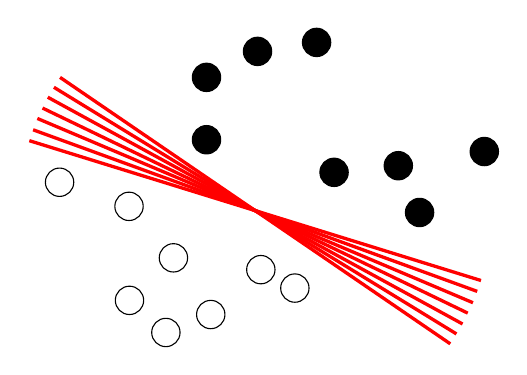
\begin{tikzpicture}[scale=0.6]
		\draw[fill=black] (6.98, -2.04) circle (0.3);
		\draw[fill=black] (6.53, -1.05) circle (0.3);
		\draw[fill=black] (8.35, -0.75) circle (0.3);
		\draw[fill=black] (5.17, -1.19) circle (0.3);
		\draw[fill=black] (2.47, -0.50) circle (0.3);
		\draw[fill=black] (4.80, 1.56) circle (0.3);
		\draw[fill=black] (3.55, 1.37) circle (0.3);
		\draw[fill=black] (2.47, 0.82) circle (0.3);
		\draw[fill=white] (1.77, -3) circle (0.3);
		\draw[fill=white] (1.61, -4.58) circle (0.3);
		\draw[fill=white] (0.83, -1.91) circle (0.3);
		\draw[fill=white] (-0.64, -1.40) circle (0.3);
		\draw[fill=white] (3.62, -3.25) circle (0.3);
		\draw[fill=white] (4.34, -3.64) circle (0.3);
		\draw[fill=white] (2.56, -4.20) circle (0.3);
		\draw[fill=white] (0.84, -3.90) circle (0.3);
		
		\draw[red, very thick] (-1.28, -0.52) -- (8.28, -3.48);
		\draw[red, very thick] (-1.20, -0.29) -- (8.20, -3.71);
		\draw[red, very thick] (-1.11, -0.05) -- (8.11, -3.95);
		\draw[red, very thick] (-1.00, 0.17) -- (8.00, -4.17);
		\draw[red, very thick] (-0.89, 0.40) -- (7.89, -4.40);
		\draw[red, very thick] (-0.76, 0.61) -- (7.76, -4.61);
		\draw[red, very thick] (-0.63, 0.82) -- (7.63, -4.82);	
	\end{tikzpicture}
\end{center}

\paragraph{Problème}
Il peux exister une multitude d'hyperplan qui séparent les données en deux. On aimerait bien avoir un algorithme qui converge vers un seul hyperplan. Il y a même pire puisqu'on peut définir l'hyperplan à un facteur près. $(x, b)$ et $(\lambda w, \lambda b)$ définissent le même hyperplan.

\paragraph{Solution}
Une solution consiste à fixer la marge fonctionnelle à être 1. C'est à dire :
$$ \left\{ \begin{matrix}
\langle w, x_+ \rangle + b & = & 1 \\
- \left( \langle w, x_- \rangle + b \right) & = & 1
\end{matrix} \right. $$
Cela permet de régler le problème de la définition de l'hyperplan à un facteur près. Cela oblige aussi à que la marge avec les point de la classe + soit la même que celle avec les points de la classe -. Pour régler le problème de la multitude d'hyperplans qui conviennent on maximise la marge géométrique. La marge géométrique est :
$$ \gamma = \frac{1}{\| w \|_2} \left( \langle w, x_+ \rangle + b \right) = - \frac{1}{\| w \|_2^2} \left( \langle w, x_- \rangle + b \right) $$
Avec la contrainte que nous nous somme fixé, on obtient :
$$ \gamma = \dfrac{1}{\| w \|_2} $$

\paragraph{Primal}
Le problème primal est alors le suivant. Étant donné un ensemble d'entraînement $T = \{ (x_i, y_i) \}_{i=1}^n$ linéairement séparable. L'hyperplan de plus grande marge est la solution du problème d'optimisation :
\begin{center}
	\fbox{ \parbox{6cm}{
		$$ \min_{w, b} \, \dfrac{1}{2} \| w \|_2^2 $$
		\vspace{-4mm}
		$$ \text{s.t. } \forall \, 1 \leqslant i \leqslant n, \, y_i \left( \langle w, x_i \rangle + b \right) \geqslant 1 $$
	} }
\end{center}
Par stricte convexité la solution est unique. Mais avec cette formulation on ne peut pas utiliser l'astuce du noyau. On doit une nouvelle fois passer par le dual. Comme le problème est convexe on dispose du théorème de dualité forte.

\paragraph{Dual}
Le lagrangien de notre problème est le suivant :
$$ L(w, b, \alpha) = \dfrac{1}{2} \| w \|_2^2 + \sum_{i=1}^{n} \alpha_i \left( 1 - y_i \left( \langle w, x_i \rangle + b \right) \right) $$
La fonction dual à maximiser est :
$$ g(\alpha) = \inf_{w, b} L(w, b, \alpha) $$
On calcule alors le gradient de $L$ par rapport à $w$ et par rapport à $b$ qui doit être nul.
$$ \dfrac{\partial L(w, b, \alpha)}{\partial w} = w - \sum_{i = 1}^{n} y_i \alpha_i x_i = 0 $$
$$ \dfrac{\partial L(w, b, \alpha)}{\partial b} = - \sum_{i = 1}^{n} y_i \alpha_i = 0 $$
Ainsi on obtient les égalités suivantes :
$$ w = \sum_{i = 1}^{n} y_i \alpha_i x_i \qquad \text{et} \qquad \sum_{i = 1}^{n} y_i \alpha_i = 0 $$
On utilise ces deux égalités dans $L$ :
$$ \begin{array}{lll}
L(w, b, \alpha)
& = & \displaystyle \frac{1}{2} \| w \|_2^2 + \sum_{i=1}^{n} \alpha_i \left( 1 - y_i \left( \langle w, x_i \rangle + b \right) \right) \\
& = & \displaystyle \dfrac{1}{2} \sum_{i, j = 1}^n y_i y_j \alpha_i \alpha_j \langle x_i, x_j \rangle \, - \, \sum_{i, j = 1}^n y_i y_j \alpha_i \alpha_j \langle x_i, x_j \rangle \, - \, b \sum_{i = 1}^n y_i \alpha_i \, + \, \sum_{i=1}^{n} \alpha_i \\
& = & \displaystyle \sum_{i=1}^{n} \alpha_i \, - \, \dfrac{1}{2} \sum_{i, j = 1}^n y_i y_j \alpha_i \alpha_j \langle x_i, x_j \rangle
\end{array} $$
Le problème dual est alors le suivant :
$$ \max_\alpha \, g(\alpha) = \sum_{i=1}^{n} \alpha_i \, - \, \dfrac{1}{2} \sum_{i, j = 1}^n y_i y_j \alpha_i \alpha_j \langle x_i, x_j \rangle $$
\vspace{-3mm}
$$ \text{s.t. } \left\{ \begin{array}{l}
	\sum_{i=1}^{n} y_i \alpha_i = 0 \\
	\alpha \succeq 0
\end{array} \right. $$
Pour retrouver les variables du primal à partir de notre solution dual optimal $\alpha^*$ on peut dans un premier temps utiliser l'équation trouvé plus haut :
$$ w^* = \sum_{i = 1}^{n} y_i \alpha_i^* x_i $$
D'après des résultats bien connus de complementary slackness, on a :
$$ \alpha_i^* \left( y_i \left( \langle w^*, x_i \rangle + b^* \right) - 1 \right) = 0 $$
Donc si $\alpha_i^* \neq 0$ alors $x_i$ est sur la marge et on obtient :
$$ b^* = \dfrac{1}{y_i} - \langle w^*, x_i \rangle $$
De plus si $x_i$ n'est pas sur la marge alors $y_i \left( \langle w^*, x_i \rangle + b^* \right) > 1$ et donc $\alpha_i = 0$. Finalement $w$ est entièrement définie par les points qui sont sur les marges. Ces point sont appelés \textbf{vecteurs de support}. On note $SV$ l'ensemble des vecteurs de support. On a :
$$ w^* = \sum_{i \in SV} y_i \alpha_i^* x_i \qquad \text{et} \qquad h(x) = \sum_{i \in SV} y_i \alpha_i^* \langle x_i, x \rangle \, + \, b^*$$
De plus avec cette formulation on peut utiliser l'astuce du noyau !!!
\begin{center}
	\fbox{ \parbox{8cm}{
			$$ \max_\alpha \, g(\alpha) = \sum_{i=1}^{n} \alpha_i \, - \, \dfrac{1}{2} \sum_{i, j = 1}^n y_i y_j \alpha_i \alpha_j K(x_i, x_j) $$
			\vspace{-3mm}
			$$ \text{s.t. } \left\{ \begin{array}{l}
			\sum_{i=1}^{n} y_i \alpha_i = 0 \\
			\alpha \succeq 0
			\end{array} \right. $$
	} }
\end{center}
La fonction de classification est alors la suivante :
$$ h(x) = \sum_{i \in SV} y_i \alpha_i^* K(x_i, x) \, + \, b^* $$

\sect{SVM à marge souple}

La SVM à marges dures a de gros problèmes. Elle ne fonctionne que si les données sont linéairement séparables ce qui n'est pas souvent le cas. Si les données sont bruités on peut obtenir des valeurs aberrantes qui mettront en échec notre modèle. On doit donc trouver un compromis entre accepté que des points soient dans la marge et la dureté de notre marge. \\

On introduit alors une marge souple avec la norme 1 :
$$ \min_{w, b, \xi}~\dfrac{1}{2} \| w \|_2^2 + C \sum_{i = 1}^n \xi_i $$
\vspace{-4mm}
$$ \text{s.t. } \left\{ \begin{array}{lll}
\forall \, 1 \leqslant i \leqslant n & y_i \left( \langle w, x_i \rangle + b \right) \geqslant 1 - \xi_i \\
 & \xi \succeq 0
\end{array} \right. $$
$C$ contrôle la pénalité que l'on donne aux points qui violent la marge. Lorsque $C$ tend vers l'infini on se retrouve dans le cas de la SVM à marges dures.
\begin{itemize}
	\item Si $\xi_i = 0$ alors $x_i$ satisfait la marge.
	\item Si $0 < \xi_i < 1 $ alors $x_i$ ne satisfait pas la marge mais est bien classé.
	\item Si $1 < \xi_i$ alors $x_i$ n'est pas bien classé.
\end{itemize}

\paragraph{Dual}
Voici notre nouveau lagrangien :
$$ L(w, b, \xi, \alpha, \beta) = \dfrac{1}{2} \| w \|_2^2 + C \sum_{i = 1}^n \xi_i + \sum_{i=1}^{n} \alpha_i \left( 1 - \xi_i - y_i \left( \langle w, x_i \rangle + b \right) \right) - \sum_{i = 1}^n \beta_i \xi_i $$
On étudie une nouvelle le gradient de $L$ par rapport à $w$, $b$ et $\xi$ :
$$ \dfrac{\partial L(w, b, \xi, \alpha, \beta)}{\partial w} = w - \sum_{i = 1}^{n} y_i \alpha_i x_i = 0 $$
$$ \dfrac{\partial L(w, b, \xi, \alpha, \beta)}{\partial b} = - \sum_{i = 1}^{n} y_i \alpha_i = 0 $$
$$ \dfrac{\partial L(w, b, \xi, \alpha, \beta)}{\partial \xi} = C \mathbbm{1} - \alpha - \beta = 0 $$
On obtient alors les égalités suivantes :
$$ w = \sum_{i = 1}^{n} y_i \alpha_i x_i \qquad \sum_{i = 1}^{n} y_i \alpha_i = 0 \qquad \text{et} \qquad \beta_i = C - \alpha_i $$
On substitue ensuite dans $L$ :
$$ \begin{array}{lll}
L(w, b, \alpha)
& = & \displaystyle \dfrac{1}{2} \| w \|_2^2 + C \sum_{i = 1}^n \xi_i + \sum_{i=1}^{n} \alpha_i \left( 1 - \xi_i - y_i \left( \langle w, x_i \rangle + b \right) \right) - \sum_{i = 1}^n \beta_i \xi_i \\
& = & \displaystyle \sum_{i=1}^{n} \alpha_i \, - \, \dfrac{1}{2} \sum_{i, j = 1}^n y_i y_j \alpha_i \alpha_j \langle x_i, x_j \rangle \, + \, \sum_{i = 1}^n \xi_i \left( C - \alpha_i - \beta_i \right) \\
& = & \displaystyle \sum_{i=1}^{n} \alpha_i \, - \, \dfrac{1}{2} \sum_{i, j = 1}^n y_i y_j \alpha_i \alpha_j \langle x_i, x_j \rangle
\end{array} $$
Finalement le problème dual est le suivant :
$$ \max_\alpha \, g(\alpha, \beta) = \sum_{i=1}^{n} \alpha_i \, - \, \dfrac{1}{2} \sum_{i, j = 1}^n y_i y_j \alpha_i \alpha_j \langle x_i, x_j \rangle $$
\vspace{-3mm}
$$ \text{s.t. } \left\{ \begin{array}{l}
\sum_{i=1}^{n} y_i \alpha_i = 0 \\
C - \alpha_i - \beta_i = 0 \\
\alpha \succeq 0 \\
\beta \succeq 0
\end{array} \right. $$
En simplifiant un peu et en ajoutant un noyau on obtient :
\begin{center}
	\fbox{ \parbox{8cm}{
			$$ \max_\alpha \, g(\alpha) = \sum_{i=1}^{n} \alpha_i \, - \, \dfrac{1}{2} \sum_{i, j = 1}^n y_i y_j \alpha_i \alpha_j K(x_i, x_j) $$
			\vspace{-3mm}
			$$ \text{s.t. } \left\{ \begin{array}{l}
			\sum_{i=1}^{n} y_i \alpha_i = 0 \\
			0 \leqslant \alpha_i \leqslant C
			\end{array} \right. $$
	} }
\end{center}
Désormais les poids $\alpha_i$ sur les $x_i$ pour définir $w$ sont bornés.